% !TEX TS-program = XeLaTeX
% use the following command:
% all document files must be coded in UTF-8
\documentclass[portuguese]{textolivre}
% build HTML with: make4ht -e build.lua -c textolivre.cfg -x -u article "fn-in,svg,pic-align"

\journalname{Texto Livre}
\thevolume{16}
%\thenumber{1} % old template
\theyear{2023}
\receiveddate{\DTMdisplaydate{2023}{4}{28}{-1}} % YYYY MM DD
\accepteddate{\DTMdisplaydate{2023}{7}{12}{-1}}
\publisheddate{\DTMdisplaydate{2023}{9}{1}{-1}}
\corrauthor{Karoline Santos Rodrigues}
\articledoi{10.1590/1983-3652.2023.45997}
%\articleid{NNNN} % if the article ID is not the last 5 numbers of its DOI, provide it using \articleid{} commmand 
% list of available sesscions in the journal: articles, dossier, reports, essays, reviews, interviews, editorial
\articlesessionname{articles}
\runningauthor{Rodrigues e Rodrigues} 
%\editorname{Leonardo Araújo} % old template
\sectioneditorname{Daniervelin Pereira}
\layouteditorname{Thaís Coutinho}

\title{A inteligência artificial na educação: os desafios do ChatGPT}
\othertitle{Artificial intelligence in education: the challenges of ChatGPT}
% if there is a third language title, add here:
%\othertitle{Artikelvorlage zur Einreichung beim Texto Livre Journal}

\author[1]{Olira Saraiva Rodrigues~\orcid{0000-0003-2371-3030}\thanks{Email: \href{mailto:ksr.karol@gmail.com}{ksr.karol@gmail.com}}}
\author[1]{Karoline Santos Rodrigues~\orcid{0000-0002-5139-9950}\thanks{Email: \href{mailto:olira.rodrigues@ueg.br}{olira.rodrigues@ueg.br}}}
\affil[1]{Universidade Estadual do Goiás, Programa de Pós-graduação Interdisciplinar em Educação, Linguagem e Tecnologias, Anápolis, Goiás, Brasil.}

\addbibresource{article.bib}
% use biber instead of bibtex
% $ biber article

% used to create dummy text for the template file
\definecolor{dark-gray}{gray}{0.35} % color used to display dummy texts
\usepackage{lipsum}
\SetLipsumParListSurrounders{\colorlet{oldcolor}{.}\color{dark-gray}}{\color{oldcolor}}

% used here only to provide the XeLaTeX and BibTeX logos
\usepackage{hologo}

% if you use multirows in a table, include the multirow package
\usepackage{multirow}

% provides sidewaysfigure environment
\usepackage{rotating}

% CUSTOM EPIGRAPH - BEGIN 
%%% https://tex.stackexchange.com/questions/193178/specific-epigraph-style
\usepackage{epigraph}
\renewcommand\textflush{flushright}
\makeatletter
\newlength\epitextskip
\pretocmd{\@epitext}{\em}{}{}
\apptocmd{\@epitext}{\em}{}{}
\patchcmd{\epigraph}{\@epitext{#1}\\}{\@epitext{#1}\\[\epitextskip]}{}{}
\makeatother
\setlength\epigraphrule{0pt}
\setlength\epitextskip{0.5ex}
\setlength\epigraphwidth{.7\textwidth}
% CUSTOM EPIGRAPH - END

% LANGUAGE - BEGIN
% ARABIC
% for languages that use special fonts, you must provide the typeface that will be used
% \setotherlanguage{arabic}
% \newfontfamily\arabicfont[Script=Arabic]{Amiri}
% \newfontfamily\arabicfontsf[Script=Arabic]{Amiri}
% \newfontfamily\arabicfonttt[Script=Arabic]{Amiri}
%
% in the article, to add arabic text use: \textlang{arabic}{ ... }
%
% RUSSIAN
% for russian text we also need to define fonts with support for Cyrillic script
% \usepackage{fontspec}
% \setotherlanguage{russian}
% \newfontfamily\cyrillicfont{Times New Roman}
% \newfontfamily\cyrillicfontsf{Times New Roman}[Script=Cyrillic]
% \newfontfamily\cyrillicfonttt{Times New Roman}[Script=Cyrillic]
%
% in the text use \begin{russian} ... \end{russian}
% LANGUAGE - END

% EMOJIS - BEGIN
% to use emoticons in your manuscript
% https://stackoverflow.com/questions/190145/how-to-insert-emoticons-in-latex/57076064
% using font Symbola, which has full support
% the font may be downloaded at:
% https://dn-works.com/ufas/
% add to preamble:
% \newfontfamily\Symbola{Symbola}
% in the text use:
% {\Symbola }
% EMOJIS - END

% LABEL REFERENCE TO DESCRIPTIVE LIST - BEGIN
% reference itens in a descriptive list using their labels instead of numbers
% insert the code below in the preambule:
%\makeatletter
%\let\orgdescriptionlabel\descriptionlabel
%\renewcommand*{\descriptionlabel}[1]{%
%  \let\orglabel\label
%  \let\label\@gobble
%  \phantomsection
%  \edef\@currentlabel{#1\unskip}%
%  \let\label\orglabel
%  \orgdescriptionlabel{#1}%
%}
%\makeatother
%
% in your document, use as illustraded here:
%\begin{description}
%  \item[first\label{itm1}] this is only an example;
%  % ...  add more items
%\end{description}
% LABEL REFERENCE TO DESCRIPTIVE LIST - END


% add line numbers for submission
%\usepackage{lineno}
%\linenumbers

\begin{document}
\maketitle

\begin{polyabstract}
\begin{abstract}
Para discutir os impactos da difusão do acesso às plataformas de modelos de linguagem na educação, este estudo aponta para questões metodológicas e substantivas em torno da Inteligência Artificial (IA) generativa para o campo de humanidades digitais, que tem preocupado educadores, principalmente do Ensino Superior, em situações como plágio, desenvolvimento crítico e criatividade na textualidade contemporânea. Assim, o estudo tem como objetivo refletir, com base na Teoria Crítica da Tecnologia de Andrew Feenberg, como a IA pode ser potencializada frente ao embaraço aversivo comum ao que exige mudanças. Metodologicamente, a pesquisa é de natureza qualitativa, exploratória e o estudo apropria-se de uma pesquisa bibliográfica, cujas contribuições inerentes à concepção de IA têm base nas produções de \textcite{2022kaufman} e \textcite{santaella2021humanos, santaella2023inteligencia}, que servem como premissa para relacionar as problematizações da IA com a Teoria Crítica da Tecnologia de \textcite{feenberg2003, feenberg2004}. Dados apontam para duas vertentes: a primeira que situa a IA generativa como evento a ser inibido das instituições de ensino, devido à falta de regulamentações éticas, e outra que orienta potencializar o uso desses produtos com finalidade crítica, na perspectiva de inteligência aumentada. Em suma, o estudo aponta que a IA do tipo generativa é um campo que carece de regulamentações, mas que pode ser conduzida de maneira coletiva, principalmente dentro das Instituições de Ensino Superior, que têm o potencial de discutir essas questões de maneira crítica e com possibilidade de efeito de ação social, a considerar a tecnologia um estilo de vida.

\keywords{Inteligência artificial \sep \emph{Chatbots} \sep Inteligência aumentada \sep Filosofia da tecnologia \sep ChatGPT}
\end{abstract}

\begin{english}
\begin{abstract}
To discuss the impacts of the diffusion of access to language model platforms in education, this study points to methodological and substantive issues around generative Artificial Intelligence (AI) for the field of digital humanities, which has concerned educators, mainly in Higher Education, in situations such as plagiarism, critical development and creativity in contemporary textuality. Thus, the study aims to reflect, based on Andrew Feenberg's Critical Theory of Technology, how AI can be enhanced in the face of the common aversive embarrassment that requires changes. Methodologically, the research is of a qualitative, exploratory nature and the study takes advantage of a bibliographical research, whose inherent contributions to the conception of AI are based on the productions of \textcite{2022kaufman} and \textcite{santaella2021humanos, santaella2023inteligencia}, which serve as a premise for to relate AI problematizations with \textcite{feenberg2003, feenberg2004} Critical Theory of Technology. Data point to two aspects: the first one that places generative AI as an event to be inhibited by educational institutions, due to the lack of ethical regulations; and the other that suggests to enhance the use of these products with a critical purpose, in the perspective of increased intelligence. In short, the study points out that generative AI is a field that lacks regulations, but that can be conducted collectively, mainly within Higher Education Institutions, which have the potential to discuss these issues critically and with the possibility of social action effect, to consider technology a way of life.

\keywords{Artificial intelligence \sep Chatbots \sep Increased intelligence \sep Philosophy of technology \sep ChatGPT}
\end{abstract}
\end{english}
% if there is another abstract, insert it here using the same scheme
\end{polyabstract}

\section{Introdução}

Estudos de natureza política, econômica e social, direcionados ao mundo digital, denotam um apreço maior de pesquisadores e de esferas governamentais e se mostram desafiadores no contexto educacional. Frente a essa situação, \textcite{santaella2021humanos} alerta para a preocupação em se discutir e em se refletir sobre as linguagens da cibercultura. Para esse movimento, a autora traz a compreensão de que o ciberespaço é o lugar onde se habita as informações cada vez mais \emph{on/offline} e as práticas sociais que envolvem esses espaços comunicacionais denominam-se cibercultura, que, na atualidade, tomam novas modelações habitadas pelo agigantamento de dados informacionais da \emph{web 4.0}.

Na fase da \emph{web} 4.0, a cibercultura é compreendida no agigantamento de dados sob a estrutura de "\emph{big data}, algoritmos de IA e a mais recente generalização, a datificação, considerada como um novo paradigma na ciência e na sociedade" \apud{dijck_data_2017}[p. 40, grifos da autora]{santaella2021humanos}. Resultante desse envolvimento humano/máquina, temos a datificação que, segundo \textcite{santaella2021humanos}, refere-se à transformação da ação social em dados on-line quantificados, permitindo, assim, o monitoramento algorítmico dos dados em tempo real e análise preditiva. O termo ainda está relacionado ao rastreamento de informações sobre o comportamento humano que são explorados por empresas e por agências governamentais, por meio da Inteligência Artificial (IA).

Um dos grandes desafios de relacionar a IA na área de humanidades é a complexidade em compreender que suas discussões não envolvem técnicas ou estratégias positivistas ou instrumentalistas. Desse modo, levantamos a seguinte problemática: a ferramenta \emph{ChatGPT}, produto da IA, é uma ameaça ou um desafio para a educação? Refletir sobre o comportamento de aversão a algoritmos \cite{feenberg2003, 2022kaufman} ou sobre as possibilidades de inteligência aumentada \cite{santaella2023inteligencia} exige um olhar mais complexo para questões sociais que permeiam o desenvolvimento e a inovação no contexto educacional.

A discussão das tecnologias na área das ciências humanas requer o entendimento de que as práticas sociais, suas relações com novos meios e mídias, é que moldam novas linguagens e novas relações. Metodologicamente, a proposta do estudo apresenta uma abordagem qualitativa e exploratória em seus objetivos, apropriando-se de uma pesquisa bibliográfica como procedimento para uma análise crítica acerca do tema. A investigação tem por objetivo refletir, com base na Teoria Crítica da Tecnologia de \textcite{feenberg2003, feenberg2004}, como a IA pode ser potencializada no contexto do Ensino Superior. Para desenvolvê-lo, buscamos conceituar a IA a partir do seu ciclo histórico, explanar sobre as diferenças da inteligência humana e IA para fundamentar uma base de complementariedade entre ambas e relacionar as problematizações oriundas do \emph{ChatGPT} com a perspectiva crítica, compreendendo a tecnologia como estilo de vida.

Este estudo apresenta um recorte teórico sobre Inteligência Artificial em \textcite{2022kaufman} e \textcite{santaella2021humanos, santaella2023inteligencia}, relacionando as problematizações pontuadas por \textcite{marques2023}, \textcite{demoraes2023}, com a Teoria Crítica da Tecnologia com base em \textcite{feenberg2003, feenberg2004}.

De modo a privilegiar a leitura e a organização lógica textual, primeiro desenvolveremos nossa reflexão a partir da explanação de popularização da IA na sociedade contemporânea. Em seguida, levantamos uma discussão sobre inteligência humana e IA. Nesse sentido, prosseguimos com a Teoria Crítica da Tecnologia de \textcite{feenberg2003, feenberg2004} para analisar como as inquietações frente ao uso das tecnologias na Educação tem se tornado um desafio que sugere potencializar a inteligência humana.
 

\section{Porque Inteligência Artificial agora?}

A expressão Inteligência Artificial (IA) remonta à década de 1950 \cite{santaella2023inteligencia} e, com seus altos e baixos, vem habitando nosso imaginário com narrativas distópicas de ficção científica, aversão ou solucionador de problemas diversos. Esse tipo de tecnologia tem se aproximado do cotidiano desde a otimização de serviços bancários por aplicativos de \emph{smartphones} até artefatos que dialogam conosco, buscando a semelhança com a linguagem humana, como a assistente de inteligência \emph{smart home} Alexa, da Amazon.

Optamos por trazer um breve recorte histórico do ciclo de vida da IA, por meio de dados levantados pelo \textcite{google} (\emph{Google Ngram}), cujo gráfico (\Cref{fig1}) apresenta uma curva de períodos em que produções acadêmicas estiveram em evidência, incluindo livros e artigos. Trata-se de uma “[...] ferramenta de pesquisa baseada na análise de milhares de livros digitalizados [...] estendem os limites da pesquisa quantitativa rigorosa para uma ampla gama de novos fenômenos que abrangem as ciências sociais e as humanidades” \cite[p. 125]{massaroo2020} . Neste estudo, o \emph{Ngram} é uma ferramenta útil para uma abordagem exploratória sobre o contexto histórico da IA, a fim de compreender os períodos mais tendenciosos e os de refluxo sobre o tema.

\begin{figure}[htbp]
\centering
\begin{minipage}{1\textwidth}
 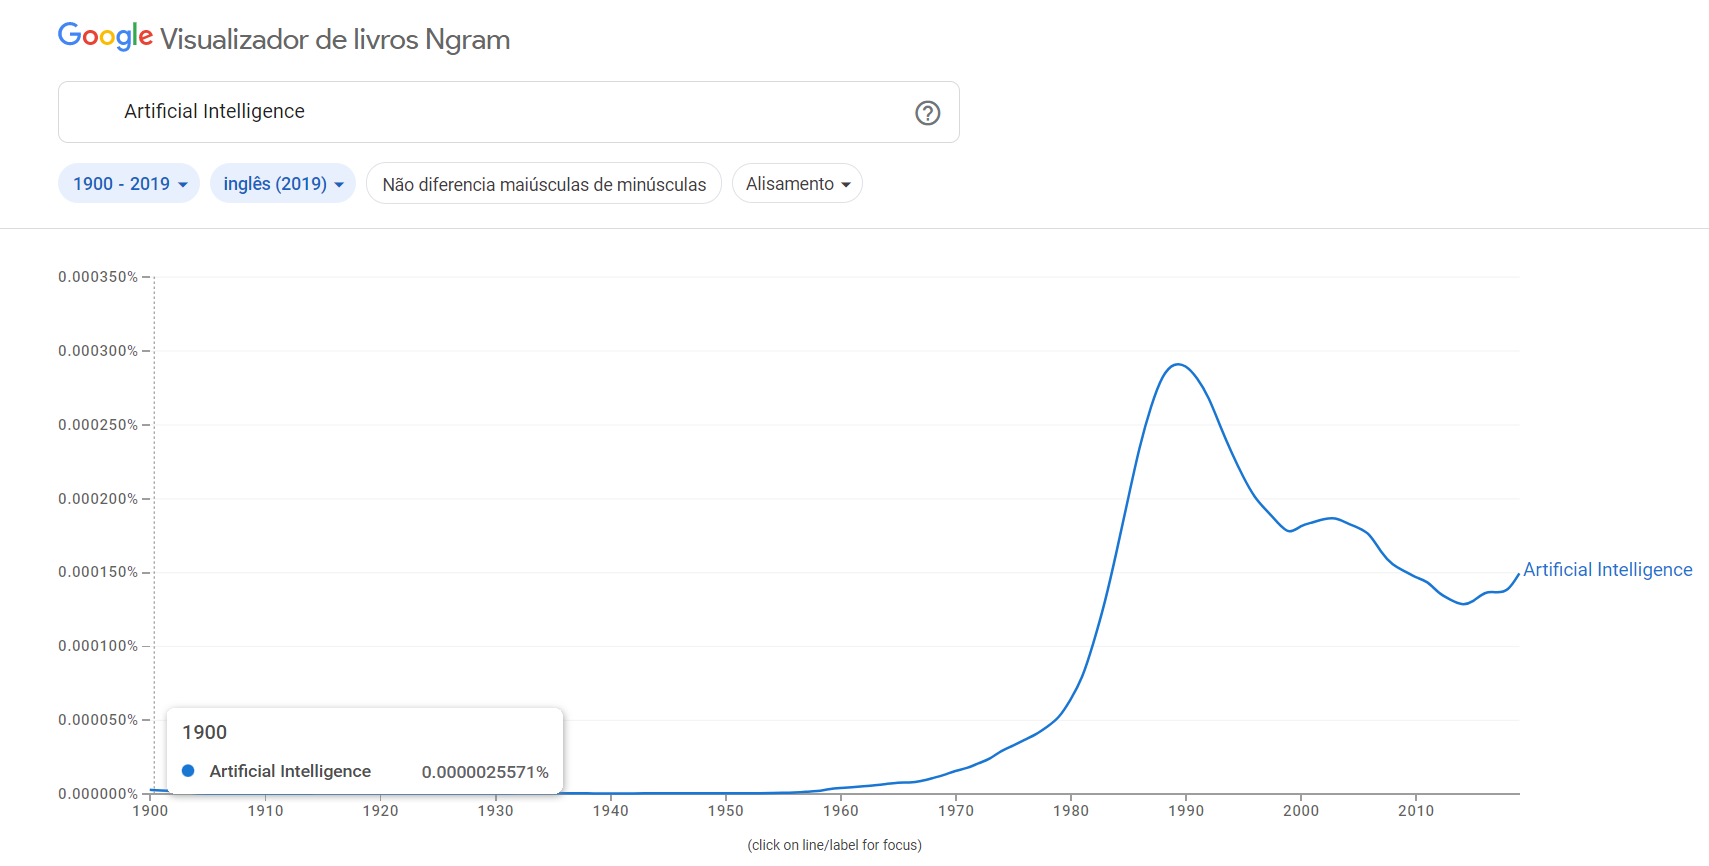
\includegraphics[width=\textwidth]{Fig1.png}
 \caption{Pesquisa sobre o termo Inteligência Artificial}
 \label{fig1}
 \source{Google Ngram Viewer, 2023.}
\end{minipage}
\end{figure}

Os dados foram extraídos do período do ano de 1900-2019, pois, curiosamente, observaram-se indícios remotos sobre a IA anteriores à década de 1950, sendo esse o período do seu surgimento indicado nas obras das autoras \textcite{2022kaufman} e \textcite{santaella2023inteligencia}.

Embora a expressão Inteligência Artificial tenha surgido no final da década de 1950, discutia-se sobre a inteligência das máquinas desde a década de 1900, quando pioneiros, como Norbert Wiener (1894-1964), propunham que a inteligência pode ser simulada por máquinas \cite{ribas2020}, não sendo uma exclusividade dos humanos \cite{santaella2023inteligencia}.

Se quisermos explorar em um contexto mais filosófico, podemos até aprofundar em Descartes (1596-1650) essa promissora discussão entre máquinas e inteligência, que integra as principais críticas sobre a influência da tecnologia na sociedade contemporânea. O filósofo abordava a relação sobre a inteligência humana produzir máquinas, “[...] pois podemos muito bem conceber uma máquina feito de tal maneira que emite palavras, e até mesmo as profere sobre ações corporais [...]\footnote{\emph{For we can well conceive of a machine made in such a way that it emits words, and even utters them about bodily actions} [...] \cite[p. 57]{mclean2006}}” \cite[p. 57, tradução nossa]{mclean2006}. Um discurso futurístico à época, mas que se mostra tão presente ao validar o potencial da inteligência humana.

Ao analisar as obras de \textcite{2022kaufman} e \textcite{santaella2023inteligencia} e relacioná-las ao gráfico representado na \Cref{fig1}, pode-se inferir que o descompasso econômico-social de acesso às redes de computadores para a sociedade das décadas de 50 e de 60 contribuiu para o baixo financiamento desse tipo de tecnologia. É nesse período que, segundo \textcite{santaella2023inteligencia}, a IA era alimentada por dados de especialistas de áreas específicas, assim, a possibilidade de coletar informações de diferentes áreas demandava um investimento alto, com promessas de resultados incertos. 

Ao analisar o contexto do surgimento da expressão IA e seu nível de produção acadêmica, é possível observar um refluxo sobre a temática até a década de 1970 e seu ressurgimento em 2010. O termo que se retrai nos anos de 1970 começa a ressurgir na década seguinte, que, segundo \textcite{2022kaufman}, se justifica com a chegada de sistemas que reproduziam regras usadas por especialistas em domínios práticos. É então a partir da década de 1990, com a construção de carros autônomos e com o acesso doméstico às redes de computadores, que o assunto recebe mais ênfase em discussões científicas, somado às obras de ficção científica que popularizou a IA de categoria geral \cite{2022kaufman, santaella2023inteligencia}. Posteriormente o termo IA passa, então, por um novo declínio e retoma o auge no século XXI, com o que ficou conhecido como \emph{redes neurais artificiais profundas}, que logo se tornou uma subárea importante da IA no ano de 2010, conhecida como \emph{deep learning} ou \emph{aprendizagem profunda}. Segundo \textcite{2022kaufman} e \textcite{santaella2023inteligencia}, o termo profunda indica que há muitas camadas de algoritmos e que são desenvolvidas pela área de aprendizagem de máquinas, responsável por ensinar o computador a realizar tarefas a partir de dados, de instruções e de textos.

Cabe um recorte breve para explicar o que são redes neurais artificiais. De forma geral, essas redes assemelham-se às sinapses cerebrais humanas. \textcite[p. 6]{2022kaufman} explica que:

\begin{quote}
    [...] redes neurais artificiais procuram reproduzir computacionalmente alguns aspectos do sistema nervoso humano, combinando unidades de processamento simples (os “neurônios artificiais”) em camadas que se ligam de forma inspirada nas sinapses do cérebro humano \cite[p. 6]{2022kaufman}.
\end{quote}

Ou seja, a máquina reconhece os padrões e cria relações entre os dados coletados. E respondendo à nossa pergunta que intitula esse item – \emph{Por que IA agora?} – compartilhamos da concepção de \textcite[p. 6]{2022kaufman}, quando afirma que a busca por Inteligência Artificial “[...] depende de avanços não só na capacidade de extrair padrões de grandes massas de dados, mas também na capacidade de receber instruções complexas no tempo”. E a capacidade de solucionar problemas tão complexos, somados ao desafio de aproximar-se à linguagem humana, sem ampliar em discussões éticas e de direitos humanos, faz com que a mirada sobre esse assunto torne-se cada vez mais emergente. Nesse prisma, são os comportamentos e as práticas sociais que contribuem para as inovações das máquinas, mesmo que cada dia estejam se desenvolvendo em uma velocidade que não podemos acompanhar minuciosamente, daí a necessidade de um olhar crítico e ético que contribua para uma melhoria social e menos desigual. 

Muito se pergunta de onde a IA que se aproxima da linguagem humana compila tantos dados, cujas respostas são quase instantâneas e surpreendentes, embora se reconheça os momentos limítrofes para falhas também. Descortinando esse \emph{modus operandi}: “tecnologia gratuita em troca dos dados, esse é o acordo que permeia as plataformas e os aplicativos tecnológicos [...]” \cite[p. 301]{2022kaufman}; são esses dados que materializam os algoritmos da IA. A entrega de nossos dados pessoais no mundo digital é tão voluntária, para não dizer obrigatória, quanto aceitar automaticamente os termos e as políticas de uso dos sites e aplicativos, sem minimamente ler as normas estampadas na tela de entrada. Estamos nós automatizados? Cabe uma reflexão pessoal de conduta, sem sequer qualquer inferência científica. Para \textcite[p. 43]{2022kaufman}, “[...] a inteligência artificial implementada atualmente em larga escala deve ser encarada como parceira dos profissionais humanos nos processos de decisão [...]”. E com essa perspectiva, prosseguimos buscando contribuir com algumas observações sobre a Inteligência Artificial generativa no contexto da educação, tendo como discussão a linguagem desenvolvida pela cibercultura.

Apesar da preocupação com o futuro de profissões, como escritores, jornalistas, educadores, designers, concentrando no contexto de linguagens, a IA pode otimizar criações, inovações, comparações de dados com maiores tendências. Mesmo que nos desafie a aprendizagens outras direcionadas ao uso de plataformas digitais, a preocupação deve dar primazia à qualidade e à veracidade das informações, além da capacidade crítica dentro do contexto em que se aplica o uso de ferramentas, como o \emph{ChatGPT}. 


\subsection{O \emph{ChatGPT}: recriar sim, mas não agir por si mesmo}

As discussões em torno das IAs de categoria generativa, que conseguem criar conteúdo possivelmente original, como imagens, músicas e até mesmo textos, precedem da preocupação de semelhança ao humano. Como exemplos, podemos citar alguns produtos: o Transformador Generativo Pré-treinado\footnote{\emph{Generative Pretrained Transformer.}} (GPT-3), da OpenAI, na produção de texto; o Modelo de Linguagem para Aplicativos de Diálogo\footnote{\emph{Language Model for Dialogue Applications.}} (LaMDA), do Google, com diálogo conversacional; o DALL-E e o Midjourney, da OpenAI, ao lerem texto e produzirem imagem. Porém, ao discutirmos o que há de inteligente nesses produtos, podemos ser conduzidos a encontrar eixos de congruências para solucionar problemáticas em que a IA não alcança, como questões que envolvem senso comum, aspectos culturais, éticos, educacionais, entre outros. \textcite[p. 165]{santaella2023inteligencia}, em sua obra \emph{A Inteligência Artificial é Inteligente?}, ao explicar o conceito de IA com base em diferentes referências, situa o conceito de IA na técnica da Aprendizagem Profunda (AP), sendo o conteúdo de IA mais amplo e diverso do que nossa imaginação. 

Lançando mão do conhecimento empírico para acrescentar um conhecimento sóbrio, \textcite{santaella2023inteligencia} salienta que devemos ser cautelosos na compreensão de termos, pois,

\begin{quote}
    [...] quando pensamos no adjetivo ‘profunda’ alocado junto à aprendizagem, podemos cair no equívoco de concluir que ela é profunda em um sentido ‘filosófico’. Mas trata-se de um termo utilizado por especialista cuja terminologia ‘profunda’ está relacionada às muitas camadas em uma rede neural \cite[p. 174, grifos das autoras]{santaella2023inteligencia}.
\end{quote}

Desse modo, como indica a autora, a AP é a técnica mais comum e acessível na sociedade. Ela está presente no reconhecimento de voz, assim como no atendimento ao cliente, nos dados multidimensionais com a visão computacional e em transações de compra e venda, sem interferência humana. Após introduzir a definição, a autora situa a problemática da máquina ser inteligente ou não. E ao abordar esse contexto, neste estudo, buscamos discutir a complementariedade das linguagens da máquina e humana.

A obra citada anteriormente é constituída de uma propensão filosófica de discutir sobre inteligências humana e artificial, por meio dos conceitos de mente, pensamento e consciência. Para esse propósito, observamos um levantamento pertinente entre inteligências artificial e humana, na indicação de alguns contrapontos, a fim de que ambas as inteligências possam ser compreendidas com seus devidos valores e complementaridade. Dentro dos inúmeros potenciais da inteligência humana, destacamos algumas características de referência em \textcite{santaella2023inteligencia} ao comparar com a IA: reusamos os conceitos; produzimos compreensões e aplicações para as coisas; transferimos aprendizagem por analogia, usando novas situações e identificando outras circunstâncias que são similares para novos cenários; temos aprendizagem estatística ao processar dados; generalizamos o padrão com poucos exemplos e aplicamos; intuímos novas respostas ao aplicar uma tendência; e obtemos conhecimento por transferência e senso comum.

Já a IA apresenta características tais como: memória, em poder assimilar e correlacionar muitos pontos de dados bem mais do que os humanos; aprendizado em tarefas específicas como classificação de imagens e processamento de sons; aprendizagem não automatizada; habilidade de processar grandes quantidades de dados; dados estatísticos fortes; e identificação de padrões informacionais que otimizam tendências relevantes. Além de tudo mencionado, não sente fadiga, sono, nem procrastina \cite{kaufman2021, santaella2023inteligencia}.

A ideia do levantamento não é discutir a melhor inteligência, mas, de fato, buscar uma complementariedade que possa nos direcionar a reconhecer que as características levantadas possam somar na produção de conhecimentos. Descartes, em \emph{O Discurso sobre o método}, de 1637, afirmava que “[...] embora tais máquinas possam fazer muitas coisas tão bem ou até melhor do que qualquer um de nós, eles inevitavelmente deixariam de fazer alguns outros\footnote{[…] \emph{although such machines might do many things as well or even better than any of us, they would inevitably fail to do some others} \cite[p. 57]{mclean2006}}” \cite[p. 57, tradução nossa]{mclean2006}. Se as máquinas são consideradas mais inteligentes que os humanos, em alguns aspectos com mais agilidades, ainda somos dotados de inteligência única.

Notamos um contraponto em \textcite[p. 249-250]{2022kaufman}, quando afirma que “[...] a inteligência artificial hoje não é inteligente, não é artificial, nem objetiva e neutra. [...] Está embutida em mundos moldados por humanos que determinam o que eles fazem e como fazem”. Nesse aspecto, a autora defende um ponto de vista em que, tendo produtores humanos, a IA não pode ser inteligente, e sim manuseada, criada. Não é neutra por estar imbuída de interesses empresariais, políticos e econômicos, como afirma \textcite{feenberg2004}, quando assegura que tecnologia é ideologia. Todavia, entre os argumentos levantados por \textcite{santaella2023inteligencia} sobre IA, ter inteligência está relacionado diretamente em como a máquina aprende e apreende. Entre as explanações dos tipos de aprendizado destacados pela autora, apontam-se três que podem se observar na relação humano e máquina: aprender por exemplos, que para humanos envolve interpretação, referência e discernimento, enquanto para máquinas aprende-se com um número muito grande de exemplos; aprender por ouvir/ falar, para ambos, deve-se tolerar critérios epistemológicos vagos, memória e competência para resolução de problemas; e aprender fazendo, aprender a fazer melhor por meio da prática repetitiva.

Em um contexto contemporâneo, podemos acrescentar ainda a aprendizagem supervisionada comum à IA. Segundo \textcite[p. 180]{santaella2023inteligencia}, essa aprendizagem:

\begin{quote}
    [...] é bastante semelhante ao aprendizado humano que se dá com a supervisão de um professor. O professor apresenta alguns exemplos específicos para que o aluno memorize, e o aluno, então, deriva regras gerais a partir deles. Mas, as aprendizagens humana e animal são, em grande parte, não supervisionadas: descobrimos a estrutura do mundo observando-o, não porque nos dizem o nome de cada objeto \cite[p. 180]{santaella2023inteligencia}.
\end{quote}

Desse modo, a justificativa de que “[...] a IA é inteligente porque o computador adquiriu o potencial de aprender e tomar decisões com base nas informações que recebe” (Ibid., p. 187) e ao combinar os padrões, adquire competência de resolver problemas de maneira quantificada, que difere da maneira qualificada da inteligência humana. Trata-se de uma inteligência útil ao ambiente organizacional, que é diferente da inteligência humana, por não gerir fatores como imaginação, criatividade e emoção.

\textcite[p. 97]{levy1993tecnologias} reitera que a relação da importância da interação social para tornar a inteligência humana única, não de modo hipervalorizado, mas reconhecendo que “[...] nossa destreza em resolver certos problemas, imóveis, de olhos fechados, deriva da capacidade, aprendida, de resolvê-los fisicamente, encadeando atos reais e percepções aos sistemas semióticos fornecidos por nossa cultura”. Nesse sentido, se não proporcionarmos ambientes críticos para o uso das tecnologias, perderemos a oportunidade de contribuir para avanços humanos na educação e na sociedade, assim, a reflexão sobre as potencialidades e os efeitos negativos devem ser contemplados com sobriedade. Posto as características de inteligência humana e IA, podemos, então, conhecer alguns pontos sobre o \emph{ChatGPT}, de modo a dialogarmos com o contexto educacional.

O \emph{ChatGPT} caracteriza-se como uma IA do tipo generativa, sendo a plataforma pioneira que se popularizou desde o ano de 2015, de maneira gratuita, chegando à atualidade com sua versão melhorada, tendo possibilidade de uso gratuito ou pago. O “GPT-3, lançado em junho 2020, foi treinado com cerca de 500 bilhões de palavras” \cite[p. 244]{2022kaufman}. Trata-se de um \emph{chatbot}\footnote{\emph{Software} que conversa com linguagem natural.} que, segundo \textcite{demoraes2023}, são parceiros de discursos, que apresentam um alto grau de refinamento nas respostas fornecidas às perguntas feitas por humanos, um sistema de reconhecimento e de produção de linguagem. E, para \textcite{santaella2023inteligencia}, ao mencionar Ferrucci (2018), “[...] não fazem outra coisa a não ser combinação de textos ao olhar para ocorrências estatísticas das palavras e frases” (p. 175). 

Um sistema complexo, no sentido de que não há controle quanto à veracidade, ética e senso comum em suas respostas. Entretanto, realiza inúmeras funções baseadas em textos, como afirma \textcite[p. 6]{demoraes2023} “[...] geração e edição de texto; pesquisa, classificação e comparação textual; geração, edição e explicação de códigos de programação; geração e edição de imagens; e treinamento de modelo para caso de uso personalizado do usuário”. Entre as informações coletadas no próprio \emph{ChatGPT}, trouxe em seu autoconceito como sendo uma IA capaz de entender e processar a linguagem natural escrita e falada, com base em conhecimentos e experiências próprios, ainda considerando suas respostas como relevantes e significativas \cite{demoraes2023}.

A criação desse tipo de IA suscita discussões críticas acerca de suas implicações, para se ter clareza que a relevância e a significação são inerentes ao contexto cultural e subjetivo do usuário. Daí a necessidade de levar esse tipo de discussão para ambientes acadêmicos. Uma IA pode saber o que é relevante ou tendencioso, se não formos nós seus principais programadores?

\textcite[p. 175]{santaella2023inteligencia}, ao explanar sobre \emph{aprendizagem profunda} (AP), base da IA mais comum ao nosso cotidiano, como a tecnologia de linguagem presente no \emph{ChatGPT}, afirma que “[...] seu senso comum está perto do zero, sendo incapaz de reconhecer quando uma pergunta é ridícula”. Contudo, suas habilidades em encontrar padrões para resoluções de problemas não podem ser desvalorizadas.

\begin{quote}
    O ChatGPT e os demais programas similares, [sic.] são protótipos funcionais que anunciam o potencial para o trabalho docente. São tecnologias que devem ser conhecidas e apropriadas por alunos, professores e escolas. Virar as costas para essas mudanças é tornar-se refém das decisões de outras pessoas, que não vão parar de investir e desenvolver esses produtos \cite[p. 6]{baltar2023professores}.
\end{quote}

Ao discorrer sobre as características da inteligência humana e IA, podemos inferir que os algoritmos presentes no \emph{ChatGPT} podem recriar, com a repetição de respostas automatizadas por seus habilidosos padrões estatísticos quantificáveis, e otimizar as tendências relevantes, que devem ser analisadas de maneira cautelosa por seus usuários; mas felizmente não é uma linguagem que pode agir por si mesmo, automatizada. 


\section{A teoria crítica da tecnologia para IA}

\begin{quote}
    O ser cognoscente é uma rede complexa na qual os nós biológicos são redefinidos e interfaceados por nós técnicos, semióticos, institucionais, culturais. A distinção feita entre um mundo objetivo inerte e sujeitos-substâncias que são os únicos portadores de atividade e de luz está abolida \cite[p. 98]{levy1993tecnologias}. 
\end{quote}

Sociólogo clássico da Cultura Digital, \textcite{levy1993tecnologias} pontua que nossa formação complexa é multifacetada e única, impregnada de saberes que também são instrumentais, porém inspirada em necessidades individuais, coletivas e socioculturais. Desse modo, compartilhamos de um estilo de vida tecnológico, logo somos influenciados a otimizar nosso tempo em espaços digitais, como ingressar em redes sociais, por exemplo.

Ao discutir o empirismo da ciência e tecnologia, \textcite{feenberg2003} considera que ambas partem do pensamento racional, em que a tecnologia não está preocupada com a verdade, mas sim com a utilidade. Desse modo, a ciência busca o saber, a tecnologia, o controle. Entretanto, precisamos compreender que a tecnologia e o conhecimento técnico, unicamente instrumentalista, não contribuem efetivamente para a educação.

Na medida em que a sociedade contemporânea assume uma base tecnológica em suas práticas econômicas, políticas e sociais, inquietações surgem, e saber para onde e o porquê estamos criando e avançando com novas tecnologias, torna-se um campo para se pensar a filosofia da tecnologia.

\begin{quote}
    As metas de nossa sociedade não podem mais ser especificadas em algum tipo de conhecimento, uma \emph{techne}, ou uma episteme [...] elas permanecem como escolhas arbitrárias puramente subjetivas, e nenhuma essência nos guia. [...] Sabemos como chegar lá, mas não sabemos por que estamos indo, ou até mesmo para onde \cite[p. 5]{feenberg2003}.
\end{quote}

A saber, notamos uma humanidade fragmentada em dados, talvez guiados pela ambição de alcançar metas sem estratégias claras ou objetivas, tornamo-nos vítimas do excesso de informação e em uma corrida insana para chegar primeiro em algum lugar sem nome. Desses comportamentos, surgem debates de hipervalorização da IA ou negação exorbitante de seu uso. 

Segundo \textcite{santaella2023inteligencia}, situações relacionadas ao sensacionalismo, imaginário baseado em ficção científica e notícias não fundamentadas difundidas culturalmente, podem ser justificadas pelo fato de estarmos dialogando sobre tecnologias extremamente poderosas, cujo processo de autonomização, isto é, sistemas tecnológicos autônomos, não estão alinhados com nossos paradigmas culturais. Não estamos preparados, culturalmente falando, para grandes saltos. A aversão à tecnologia também tem lugar de fala em \textcite[p. 4]{feenberg2004}, quando afirma que “[...] mundos diferentes, que fluem dos diferentes arranjos técnicos e das diferentes posições internas a eles, privilegiam alguns aspectos do ser humano e marginalizam outros”. Podemos observar, por exemplo, quando a IA se mostra habilidosa em reconhecimento de padrões em uma situação-problema, quando usaríamos um tempo maior para identificar. Desse modo, somos privilegiados no aspecto de criar os comandos, lançar os \emph{inputs}, quando somos marginalizados na identificação de padrões com agilidade.

Apesar de o imaginário tecnológico continuar preso às imagens das ficções científicas com robôs tirânicos, ainda assim, dormimos ao silêncio dos nossos \emph{smartphones} debaixo do travesseiro, ou nos afeiçoamos à IA como companhia à mesa de refeição, ou como mentor em uma sala de estudos; enfim, de perto e outrora contida. \textcite[p. 14]{santaella2023inteligencia}, com coerência em nossos comportamentos, é pontual ao afirmar que “[...] a contradição entre o bem e o mal é indicadora do pouco entendimento que reina sobre a IA”.

Uma das principais críticas à tecnologia observada em \textcite{feenberg2004} estão relacionadas ao controle, desmundificação e automação, cujas problemáticas são contrapostas ao abordar questões relacionadas à democracia tecnológica e à teoria crítica. Para ele, não basta ampliar as formas de conhecimento, mas identificar as estruturas de poder que influenciam o conhecimento e suas aplicações. É nesse contexto que defende que a tecnologia não é neutra e deve ser discutida com seriedade nas instituições de ensino. O filósofo ainda propõe algumas contribuições com a teoria crítica da tecnologia que “alertam para os riscos e poderes inerentes à tecnologia, bem como para sua capacidade de manipulação sociocultural, revelando a necessidade de maior reflexividade e de mudança de paradigma instrumental” \cite[p. 20]{ninis2013}.

Nesse sentido, um efeito da IA, apontado por \textcite{santaella2023inteligencia}, que podemos relacionar à educação e à teoria crítica da tecnologia, está no sentido de que

\begin{quote}
    Não estamos dispostos a abdicar das facilitações pragmáticas e recompensas psíquicas que o nosso mimoso \emph{smartphone} nos propicia, saber que estamos sendo digitalmente modelados, na constituição de uma existência especular, provoca uma espécie de \emph{Unheimlich}, o inquietante estranhamento do familiar que foi estudado por Freud \cite[p. 17]{santaella2023inteligencia}.
\end{quote}

É a comum situação de que em nossas individualidades, afeiçoamo-nos à otimização de tempo, interação social e acesso à informação que as tecnologias nos proporcionam, mas, quando se amplia à discussão educacional, a tecnologia vira um corpo estranho. Apesar de todos os efeitos, para \textcite[p. 23]{santaella2023inteligencia}, a IA precisa de “[...] recortes objetivos, precisos e claramente expostos para discussão”; a ausência de tais atributos insere a discussão em um campo minado puramente crítico, sem o entendimento da complexidade do fenômeno da IA. Universidades têm levantado preocupações morais e éticas quanto ao uso de tecnologias que abrangem a IA generativa, além disso surgem preocupações outras, como desigualdades, plágio, falta de senso crítico, entraves criativos e atrofias epistêmicas.

Os desafios considerados no uso do \emph{ChatGPT}, de modo geral, são comuns aos apontados na própria tecnologia da inteligência artificial, como "enviesamento e preconceito, moderação de conteúdo ilegal ou antiético, proteção à privacidade, fake news [...]" \cite[p. 191]{2022kaufman}. Esse cenário é propício para discutir, por exemplo, a necessidade de propostas de políticas regulatórias, como baliza os estudos de \textcite{coeckelbergh2020ai}, quando aponta para a necessidade de investigar, criar e questionar as políticas no que concerne à IA.

Para \textcite[p. 83]{2022kaufman}, a partir do momento em que consideramos a aprendizagem de máquina como uma habilidade de combinação de dados algoritmos para a produção de respostas automatizadas, "coloca[-se] para a sociedade novos desafios éticos e a premência de estabelecer arcabouços legais", que protejam não apenas os indivíduos, mas também as instituições, preservando a liberdade necessária ao desenvolvimento e rigor científico.

Por ser inseparável da interferência humana, \textcite{santaella2023inteligencia} complementa também que este se torna um grande desafio que cerca a ética da IA. Nesse propósito, porque não discutir questões éticas, antes de novas invenções? \textcite[p. 2]{feenberg2004} afirma que o domínio sob as tecnologias é meramente humano, uma vez que “[...] na medida que [sic.] podemos planejar e conduzir o desenvolvimento técnico por vários processos públicos e escolhas privadas é que temos algum controle sobre nossa própria humanidade”. Mas, o que podemos observar é que questões significativas de valores são suprimidas no processo de criação de IA e essa situação requer uma análise para que esse controle não entre em colapso. 

Para as discussões dos efeitos da IA na educação, de antemão, “[...] é preciso considerar que manter-se [sic.] na visão de que o domínio dos fatos e do conhecimento é aquilo que faz uma pessoa inteligente ou preparada não passa de uma visão desproporcional da inteligência humana” \cite[p. 183]{santaella2023inteligencia}. E de acordo com a autora, nos “[...] modelos de IA capazes de escrever textos [...] não se manifesta o pensamento divergente, pois, para este, ainda é necessário o cérebro humano” (Ibid., p. 183). Não podemos ser incoerentes ou equivocados a ponto de considerar que domínio de fatos e conhecimentos é sinônimo de inteligência; desse modo, estaríamos nos comparando às máquinas.

Para \textcite[p. 10]{feenberg2003}, “[...] na teoria crítica, as tecnologias não são vistas como ferramentas, mas como estruturas para estilos de vida”. Cada vez mais digital, a sociedade tem se apropriado das tecnologias em sua vida diária, enquanto os paradigmas educacionais tentam encontrar, ou pelo menos deveriam, um ponto de equilíbrio para não coibir o ingresso desses artefatos em sala de aula.

Vejamos nas reflexões de \textcite{demoraes2023}, quando o assunto é IA generativa, com o \emph{ChatGPT}:

\begin{quote}
    alternativas têm sido pensadas por profissionais da educação para evitar que trapaças utilizando o ChatGPT sejam bem-sucedidas: aplicação de provas escritas à mão; trabalhos realizados em sala de aula; opção por provas orais, entre outros meios nos quais o ChatGPT não pode ser utilizado. Porém, mais do que proibir o uso desta tecnologia, precisamos repensar a forma como a educação pode se apropriar dela \cite[p. 4]{demoraes2023}.
\end{quote}

Outro ponto desafiador dos \emph{chatbots} de modelo de linguagem natural como o \emph{ChatGPT}, segundo \textcite[p. 40]{marques2023}, é "justamente a originalidade de suas respostas e o receio de que se transforme em uma fonte de má conduta acadêmica". Quanto às situações proeminentes de plágio no contexto educacional, uma pesquisa realizada nos Estados Unidos, pela Universidade do Estado da Pensilvânia (Penn State), sobre o uso da ferramenta \emph{ChatGPT}, aponta para indícios de plágios na construção de respostas aos usuários \cite{demoraes2023}. A pesquisa assinala, ainda, para a ocorrência de transcrições literais de textos, paráfrases e apropriação de ideias sem referência à fonte, além de ser comum a ausência de pensamento divergente \cite{santaella2023inteligencia} por se tratar de uma aprendizagem de máquina.

Desse modo, verificamos dois impactos relacionados ao acesso e ao uso de plataformas de modelos de linguagem natural que usam a inteligência artificial: o primeiro envolve questões relacionadas à regulamentação para mitigar sobre temas relacionados aos direitos autorais, às Fake News, à ética, à proteção à privacidade, etc. \cite{coeckelbergh2020ai, kaufman2021, 2022kaufman}; o segundo ponto está relacionado às más condutas acadêmicas, envolvendo situação de plágio \cite{marques2023, demoraes2023}.

Formas de se prevenir o problema de má conduta acadêmica, segundo \textcite[p. 40]{marques2023}, são a utilização de programas capazes de detectar textos de IA, como o Demonstrador de saída GPT2 "(\url{openai-openai-detector.hf.space/}) [...], o Writer AI Content Detector (\url{writer.com/ai-content-detector/}) e o Content at Scale (\url{contentatscale.ai/ai-content-detector/})", e a necessidade de treinamento de pessoas, uma vez que as máquinas estão em constante evolução. Desse modo, no espaço acadêmico, temos a possibilidade de despertar não apenas o olhar crítico nas respostas disponibilizadas por essas ferramentas, mas a habilidade em compreender e diferenciar quando o texto é elaborado por um modelo de linguagem natural. 

A pesquisa realizada pela Universidade do Estado da Pensilvânia (Penn State), nos Estados Unidos, com estudantes do Ensino Superior, aponta que, por meio de jogos, os participantes identificaram textos elaborados pelo \emph{ChatGPT}, ao observarem "o surgimento de conteúdo irrelevante, de erros lógicos, de sentenças contraditórias, de frases muito genéricas e de problemas com a gramática" \cite[p. 41]{marques2023}. Ao identificar esses pontos, consideramos sua aplicabilidade no Ensino Superior, com a finalidade de desenvolver habilidades críticas, de escrita e de textualidade, melhoria de desempenho em conteúdos específicos, desenvolvimento lógico, adensamento epistemológico, entre outros. 

Nesse contexto, há um cenário que precisa dialogar com a perspectiva da Teoria Crítica de Feenberg, pois é um choque de diferentes mundos em uma sociedade que se baseia no domínio tecnológico. \textcite{demoraes2023} ainda argumentam que novas estratégias educacionais para o uso dessa ferramenta, e outras que possam surgir, devem ser municiadas de fundo ético e efetivo, inclusive com a intervenção de poderes públicos e de responsabilidade coletiva.

Outros pontos de reflexão precisam ser ampliados no intuito de que IA, como o \emph{ChatGPT}, potencialize o conhecimento acadêmico. \textcite{2022kaufman} e \textcite{santaella2023inteligencia} levantam uma discussão importante para que possamos vislumbrar possibilidades do uso da IA sob uma perspectiva de ‘inteligência aumentada’, em realizar perguntas coerentes, com objetivos claros, escolher entre recomendações e buscar referências com comprovação científica. 

Podemos usar a IA para extrair conhecimento responsável e transparente a partir de seus inúmeros dados; porém, a primazia do senso comum sobre a veracidade e o que fazer com esses dados devem ser tomados com clareza e sobriedade, a fim de alcançar a máxima em que defende \textcite{santaella2023inteligencia}, segundo a qual “[...] conhecer os desenvolvimentos da IA deveria ser um modo de redescobrir o humano” (p. 191).

A partir dos levantamentos elucidativos apresentados neste texto, observamos que o uso de modelos de linguagem natural pode ser proposto com dinâmicas coletivas em ambientes acadêmicos, na compreensão da complexidade com que as respostas elaboradas pelas ferramentas estão relacionadas ao comportamento compartilhado em redes. De certa forma, a Teoria Crítica da Tecnologia de Feenberg auxilia na identificação das estruturas de poder que influenciam as respostas.

O trabalho colaborativo, entre docente e estudantes, ao criar e identificar textos que possuem trechos elaborados pelo \emph{ChatGPT}, possibilita discussões outras, relacionadas às questões éticas, culturais, de direitos, levantando problemáticas, tais como preconceito, racismo etc., propiciando práticas que rompam com o paradigma instrumental \cite{feenberg2004} no uso das tecnologias digitais em sala de aula. Consideramos ser este um estudo ainda incipiente no cenário brasileiro, mas que instiga reflexões e propostas futuras para avaliar, na prática, a habilidade despertada nos estudantes, sendo complementada com as tecnologias de inteligência artificial, que desafiam a educação na cultura digital.

Enfim, a compreensão acerca de como a IA tem avançado timidamente em nossas discussões transversais, em que suas habilidades não podem ser ignoradas em nossos estilos de vida, é fundamental para que possamos pensar uma educação crítica, que contribua para uma inteligência aumentada agora pelos algoritmos da IA. 


\section{Conclusão}

Como observamos, na Teoria Crítica da Tecnologia de \textcite{feenberg2003, feenberg2004}, não há neutralidade na tecnologia. Nesse sentido, \textcite{kaufman2021} e \textcite{coeckelbergh2020ai} argumentam que avançamos para questões de defender o uso ético da IA para mitigar riscos a longo prazo. A inteligência artificial não garante objetividade e neutralidade apenas por ser processada por máquinas e supostamente protegida contra erros humanos, fator observado no uso da ferramenta \emph{ChatGPT}, cujas buscas e contribuições não estão isentas de erros, aos quais necessitam de uso reflexivo, consciente e crítico, considerando o contexto e as práticas sociais.

Quando \textcite{feenberg2003} nos confronta com a realidade de que a sociedade contemporânea não está munida de metas claras, logo pensamos na velocidade desenfreada que vivemos, apontada como um sério problema por \textcite{bauman2013cultura}. A popularização da IA generativa e seu avanço desenfreado tem afetado, em âmbito educacional, questões relacionadas à ética no desenvolvimento científico, produção de valores e senso comum. Por isso, devemos confrontar, cientes de que a IA é apenas um dos tipos de inteligência em que compartilhamos nosso mundo.

Somos seres qualitativos, com potencial crítico, intuição para novas tendências e senso comum, que é resultado de experiências socioculturais. O estudo aponta que a IA é um campo que carece de regulamentações e consideramos que pode ser conduzida de maneira coletiva, principalmente dentro das Instituições de Ensino Superior, espaço com potencial para discutir tais questões, sem ingenuidade e com criticidade, na possibilidade de reverberar ações críticas no contexto social, pelo compromisso e pela responsabilidade com a sociedade que integra.

Depreendemos do percurso deste estudo que o desenvolvimento de algoritmos e de novas tecnologias na educação passa a ser uma aversão, quando nos demoramos em observar as potencialidades dos produtos que decidimos utilizar. Por outro lado, no contexto de linguagem, a IA pode, muitas vezes, indicar respostas tendenciosas, ao seguir padrões sem embasamento e referência científica, não atingindo o pensamento divergente. E é nesse entendimento que se convoca o cérebro humano e afirmamo-nos necessários, que tomamos como meta inacabada redescobrir e redirecionar o potencial humano para ações colaborativas de valorização cidadã, humanitária e tecnologicamente emancipadora. 


\printbibliography\label{sec-bib}
% if the text is not in Portuguese, it might be necessary to use the code below instead to print the correct ABNT abbreviations [s.n.], [s.l.]
%\begin{portuguese}
%\printbibliography[title={Bibliography}]
%\end{portuguese}


%full list: conceptualization,datacuration,formalanalysis,funding,investigation,methodology,projadm,resources,software,supervision,validation,visualization,writing,review
\begin{contributors}[sec-contributors]
\authorcontribution{Olira Saraiva Rodrigues}[conceptualization,review,resources]
\authorcontribution{Karoline Santos Rodrigues}[conceptualization,resources,writing]
\end{contributors}



\end{document}

